\hypertarget{stm32f4xx__hal__tim__ex_8c}{}\section{Dokumentacja pliku S\+T\+M/\+W\+D\+S\+\_\+\+Kosc\+\_\+\+Linux/\+Drivers/\+S\+T\+M32\+F4xx\+\_\+\+H\+A\+L\+\_\+\+Driver/\+Src/stm32f4xx\+\_\+hal\+\_\+tim\+\_\+ex.c}
\label{stm32f4xx__hal__tim__ex_8c}\index{S\+T\+M/\+W\+D\+S\+\_\+\+Kosc\+\_\+\+Linux/\+Drivers/\+S\+T\+M32\+F4xx\+\_\+\+H\+A\+L\+\_\+\+Driver/\+Src/stm32f4xx\+\_\+hal\+\_\+tim\+\_\+ex.\+c@{S\+T\+M/\+W\+D\+S\+\_\+\+Kosc\+\_\+\+Linux/\+Drivers/\+S\+T\+M32\+F4xx\+\_\+\+H\+A\+L\+\_\+\+Driver/\+Src/stm32f4xx\+\_\+hal\+\_\+tim\+\_\+ex.\+c}}


T\+IM H\+AL module driver. This file provides firmware functions to manage the following functionalities of the Timer Extended peripheral\+:  


{\ttfamily \#include \char`\"{}stm32f4xx\+\_\+hal.\+h\char`\"{}}\newline
Wykres zależności załączania dla stm32f4xx\+\_\+hal\+\_\+tim\+\_\+ex.\+c\+:\nopagebreak
\begin{figure}[H]
\begin{center}
\leavevmode
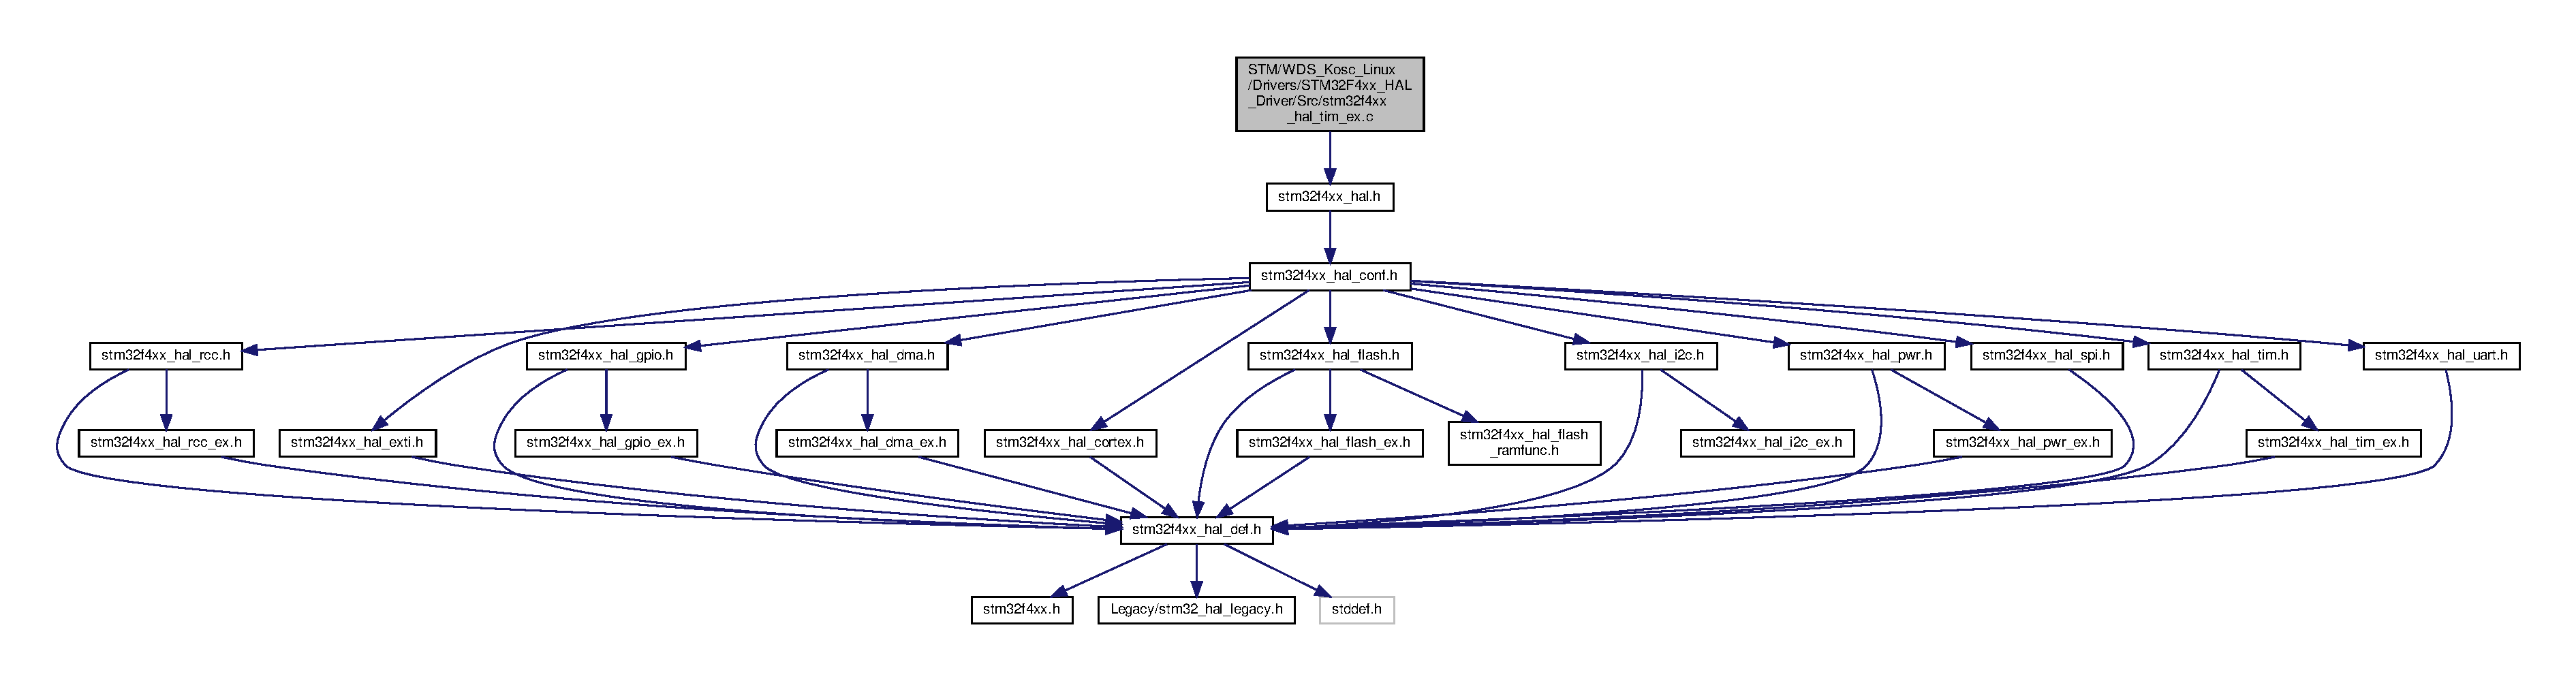
\includegraphics[width=350pt]{stm32f4xx__hal__tim__ex_8c__incl}
\end{center}
\end{figure}


\subsection{Opis szczegółowy}
T\+IM H\+AL module driver. This file provides firmware functions to manage the following functionalities of the Timer Extended peripheral\+: 

\begin{DoxyAuthor}{Autor}
M\+CD Application Team
\begin{DoxyItemize}
\item Time Hall Sensor Interface Initialization
\item Time Hall Sensor Interface Start
\item Time Complementary signal break and dead time configuration
\item Time Master and Slave synchronization configuration
\item Timer remapping capabilities configuration \begin{DoxyVerb}==============================================================================
                    ##### TIMER Extended features #####
==============================================================================
[..]
  The Timer Extended features include:
  (#) Complementary outputs with programmable dead-time for :
      (++) Output Compare
      (++) PWM generation (Edge and Center-aligned Mode)
      (++) One-pulse mode output
  (#) Synchronization circuit to control the timer with external signals and to
      interconnect several timers together.
  (#) Break input to put the timer output signals in reset state or in a known state.
  (#) Supports incremental (quadrature) encoder and hall-sensor circuitry for
      positioning purposes

          ##### How to use this driver #####
==============================================================================
  [..]
   (#) Initialize the TIM low level resources by implementing the following functions
       depending on the selected feature:
         (++) Hall Sensor output : HAL_TIMEx_HallSensor_MspInit()

   (#) Initialize the TIM low level resources :
      (##) Enable the TIM interface clock using __HAL_RCC_TIMx_CLK_ENABLE();
      (##) TIM pins configuration
          (+++) Enable the clock for the TIM GPIOs using the following function:
            __HAL_RCC_GPIOx_CLK_ENABLE();
          (+++) Configure these TIM pins in Alternate function mode using HAL_GPIO_Init();

   (#) The external Clock can be configured, if needed (the default clock is the
       internal clock from the APBx), using the following function:
       HAL_TIM_ConfigClockSource, the clock configuration should be done before
       any start function.

   (#) Configure the TIM in the desired functioning mode using one of the
       initialization function of this driver:
        (++) HAL_TIMEx_HallSensor_Init() and HAL_TIMEx_ConfigCommutEvent(): to use the
             Timer Hall Sensor Interface and the commutation event with the corresponding
             Interrupt and DMA request if needed (Note that One Timer is used to interface
             with the Hall sensor Interface and another Timer should be used to use
             the commutation event).

   (#) Activate the TIM peripheral using one of the start functions:
         (++) Complementary Output Compare : HAL_TIMEx_OCN_Start(), HAL_TIMEx_OCN_Start_DMA(), HAL_TIMEx_OC_Start_IT()
         (++) Complementary PWM generation : HAL_TIMEx_PWMN_Start(), HAL_TIMEx_PWMN_Start_DMA(), HAL_TIMEx_PWMN_Start_IT()
         (++) Complementary One-pulse mode output : HAL_TIMEx_OnePulseN_Start(), HAL_TIMEx_OnePulseN_Start_IT()
         (++) Hall Sensor output : HAL_TIMEx_HallSensor_Start(), HAL_TIMEx_HallSensor_Start_DMA(), HAL_TIMEx_HallSensor_Start_IT().\end{DoxyVerb}

\end{DoxyItemize}
\end{DoxyAuthor}
\begin{DoxyAttention}{Uwaga}

\end{DoxyAttention}
\subsubsection*{\begin{center}\copyright{} Copyright (c) 2016 S\+T\+Microelectronics. All rights reserved.\end{center} }

This software component is licensed by ST under B\+SD 3-\/\+Clause license, the \char`\"{}\+License\char`\"{}; You may not use this file except in compliance with the License. You may obtain a copy of the License at\+: opensource.\+org/licenses/\+B\+S\+D-\/3-\/\+Clause 